\section{Have Gun, Will Travel}

\begin{quotex}
Fortune favors the audacious.
\flright{\textsc{Erasmus}}

He doesn't care about proof, he doesn't care about the law, he only cares about what's right.
\flright{\textsc{re Jack Reacher}}
\end{quotex}


\paragraph{Three Soul Forces}


The three soul forces are:

\begin{itemize}


\item \textbf{Epithumos or Appetite}: The force that satisfies desires.


\item \textbf{Thumos or Passion}: The emotional elements that drives the will.

\item \textbf{Nous or Intellect}: The drive to knowledge.

\end{itemize}


In the healthy soul, the Nous will be the master over the passions and appetites. The disordered soul will be dominated by passions or desires.

\paragraph{Knowledge of the Good}


The nous does not mean the person who can write a scholarly paper with references, footnotes, etc. Rather, it is knowledge of the Good which is accessible even to those without a formal education. On the other hand, those who are capable of it, and have the opportunity, should undertake the appropriate studies; that is indicative of the desire to know the Good.

Knowledge of the Good and desire for the Good are insufficient. One must will the Good, which is a much more difficult project. Knowledge of the Good is dispassionate, disinterested, and objective. This may come in conflict with one's personal desires. There are two ways to mitigate that problem:

\begin{itemize}


\item Reduce one's property and personal needs.

\item Have an excess of property or wealth, enough to satisfy one's needs.
\end{itemize}


\paragraph{The Solitary Man}


What applies to the individual man, applies also to the City. The best City promotes the good and teaches the good. Its goal is justice. The corrupt City is unjust and is dominated by those with excessive desires, such as lust or greed. They then use the mechanism of the City for personal gain.

In such cases, often justice can be achieved by the Solitary Man, who acts from outside the system. That archetype is common in the West, going back to the Paladins of the Round Table. Although that figure was satirized in \emph{Don Quixote}, it still lives on. The colonization of the West in the USA during the 19\textsuperscript{th} century gave new life to that figure, even in Germany of all places. With the growth of the film industry, this figure has reappeared in different guises. These are the main characteristics:

\begin{itemize}


\item He is incorruptible.

\item He is solitary, having no permanent personal attachments.

\item He is experienced in the world, having previously taken part in the life of the City.

\item He is highly intelligent and knows several languages.

\item He is a great judge of human character and notices details missed by most.

\item He is the consummate fighter, skilled in martial arts and fisticuffs.

\item He is an expert in weapons, both hot and cold.

\item He is protective of women and children. The female relationship is usually chaste, although some studios, like Amazon, simply cannot restrain themselves.

\item He works outside the system. The rules and laws of society are flouted in the interests of Justice.
\end{itemize}


\paragraph{Jack Reacher}


A contemporary exemplar of the first type is Jack Reacher, based on a novel and then made into two feature films and more recently an Amazon series. Jack Reacher has no permanent address, no credit rating, and is basically invisible to the Internet. He wanders like a hobo. Of course, since corruption is ubiquitous, he will often encounter an unjust situation.

As a former member of the military police, he is knowledgeable about the laws and procedures. Through insight and force, he manages to uncover the secret movers and shakers in the City. Unburdened by the laws and rules of evidence of the City, he employs any extreme measure, even torture and extortion, to gather information. Although the authorities are exasperated by his style, he is vindicated in the end.

There is an interesting comment by the teenage female character in \emph{Jack Reacher: Never Go Back}. After Jack warned her to stay away from the street people, this was her response. ``I always go to the alpha male, because he won't hurt me. He has a younger sister, or wishes he did. The strong man won't hurt me, only the weak man will.''

\paragraph{Paladin}

\begin{wrapfigure}{rt}{.3\textwidth}
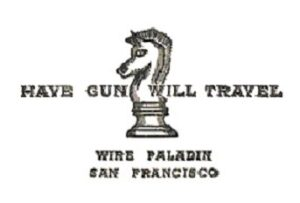
\includegraphics[width=.3\textwidth]{HaveGunWillTravel-300x203.jpg}
\end{wrapfigure}

Paladin refers to the character in the 1950s television series, \emph{Have Gun -- Will Travel}. Paladin is primarily a ``fixer'', who resolves problems for the wealthy. Nevertheless, he will still help out those who cannot afford him \emph{pro bono}.

Unlike Reacher, Paladin lives the life of a prosperous gentleman. He lives well, follow high culture, is interested in music. He is educated in the classics and Western philosophy, speaks several languages, and has a good knowledge of the Law. He knows Chinese martial arts, fisticuffs, guns, and even swords.

His business card bears the image of the Knight chess piece. In my fantasy life as a consultant, I modeled myself on this character; I would fix problems few other could. Travel took me to some desirable places, but often remote areas in the rural South. Eventually the lone wolf went out of style in favor of large consulting firms with various certifications.


\flrightit{Posted on 2022-03-13 by Cologero}

